% -*- latex -*-
%-----------------------------------------------------------------------
%;  Copyright (C) 2001
%;  Associated Universities, Inc. Washington DC, USA.
%;
%;  This program is free software; you can redistribute it and/or
%;  modify it under the terms of the GNU General Public License as
%;  published by the Free Software Foundation; either version 2 of
%;  the License, or (at your option) any later version.
%;
%;  This program is distributed in the hope that it will be useful,
%;  but WITHOUT ANY WARRANTY; without even the implied warranty of
%;  MERCHANTABILITY or FITNESS FOR A PARTICULAR PURPOSE.  See the
%;  GNU General Public License for more details.
%;
%;  You should have received a copy of the GNU General Public
%;  License along with this program; if not, write to the Free
%;  Software Foundation, Inc., 675 Massachusetts Ave, Cambridge,
%;  MA 02139, USA.
%;
%;  Correspondence concerning AIPS should be addressed as follows:
%;          Internet email: aipsmail@nrao.edu.
%;          Postal address: AIPS Project Office
%;                          National Radio Astronomy Observatory
%;                          520 Edgemont Road
%;                          Charlottesville, VA 22903-2475 USA
%-----------------------------------------------------------------------
%Body of intermediate AIPSletter for 31 December 2001

\documentclass[twoside]{article}
\usepackage{graphics}

\newcommand{\AIPRELEASE}{June 30, 2001}
\newcommand{\AIPVOLUME}{Volume XXI}
\newcommand{\AIPNUMBER}{Number 1}
\newcommand{\RELEASENAME}{{\tt 31DEC01}}
\newcommand{\OLDNAME}{{\tt 31DEC00}}
\newcommand{\NEXTNAME}{{\tt 31DEC01}}

%macros and title page format for the \AIPS\ letter.
\input LET98.MAC
%\input psfig

\newcommand{\MYSpace}{-11pt}

\normalstyle

\section{General developments in \AIPS}

\subsection{Linux news}

RedHat has released versions 7.0 and now 7.1 of their Linux system.
The good news is that version 7.1 in particular contains numerous
system improvements including the 2.4.2 kernel.  This kernel allows
\AIPS\ to read and write files larger than 2 Gbytes.  The bad news is
that both of these releases include and depend on the ``GNU compilers
version 2.96.''  The quote marks are added because the GNU compiler
group never released a version 2.96 and they have washed their hands
of this ``version'' on their web site.  We have found that the {\tt
g77} compiler appears to work on \AIPS\ but produces optimized code
that is unreliable.  {\tt IMAGR} is one of the tasks that does not
work correctly under this compiler and one should never use {\tt
IMAGR} without optimization.  There are also problems with TV window
setting, {\tt TVFLG}, and who knows what else.  We do recommend RedHat
release 7.1, but you must also install the older GNU compiler suite
version 2.95 and change your local copies of {\tt FDEFAULT.SH}, {\tt
CCOPTS.SH}, and {\tt FDOPTS.SH} to point at it.  Some other Linux
distributions also include the 2.96 compiler with the same unfortunate
results.

\subsection{Personnel changes}

Pat Murphy, because of the press of his other duties, has asked to be
relieved of all official duties in the \AIPS\ Group.  He has been a
valuable member of the Group for over ten years and he will be
missed.  Like Bill Cotton before him, he has volunteered to advise the
remaining group privately as needed.  Additional assistance with
operating system matters will now be provided by the very capable
members of the Computer Division at the Array Operations Center in
Socorro.  Please direct inquiries to {\tt daip@nrao.edu} and not to
Pat's e-mail address.

Amy Mioduszewski joined the \AIPS\ Group in Socorro in January.  She
has already had a significant impact in writing and improving a
variety of {\tt PROCEDURE}s for simplified data reduction.

\subsection{Current and future releases}

We have reinstated the old practice of having formal \AIPS\ releases,
but on an annual basis with binary releases only for Solaris and
Linux.  All architectures can do a full installation from the source
files.  The next release will be called {\tt 31DEC01} and remains under
development by the (reduced) \AIPS\ Group.  You may fetch and install
a complete copy of this version at any time.  This \Aipsletter\ is
intended to advise you of developments to date in this new release.
Having fetched {\tt 31DEC01}, you may update your installation
whenever you want either as a whole or by running the so-called
``midnight job'' which uses transaction files to copy and compile the
code selectively based on the code changes and compilations we have
done.  We expect users to take the source-only version of {\tt
31DEC01} \AIPS\ over the Internet (via \emph{anonymous} ftp).

\AIPS\ is now copyright \copyright\ 1995 through 2001 by Associated
Universities, Inc., NRAO's parent corporation, but may be made freely
available under the terms of the Free Software Foundation's General
Public License (GPL)\@.  This means that User Agreements are no longer
required, that \AIPS\ may be obtained via anonymous ftp without
contacting NRAO, and that the software may be redistributed (and/or
modified), under certain conditions.  The full text of the GPL can be
found in the \texttt{15JUL95} \Aipsletter.

\section{Improvements of interest to users in \RELEASENAME}

We expect to continue publishing the  \Aipsletter\ approximately every
six months along with the annual releases.  Despite the reduction in
personnel, there have been a surprising number of changes in {\tt
31DEC01} over the past six months.  There are five new tasks: {\tt
CHKFC} to check the contents of an {\tt IMAGR} {\tt BOXFILE}, {\tt
DEFLG} to flag data based on the level of decorrelation, {\tt SNFLG}
to flag data on a baseline basis based on phase jumps in the {\tt SN}
or {\tt CL} table, {\tt VPFLG} to make sure that all polarizations are
flagged in a sample if any are, and {\tt DRCHK} to test the
installation control files for correctness.  A new verb was written
called {\tt EPOCONV} to convert epochs in the {\tt COORDINA} adverb.
New VLBA Utility procedures are also available.

Other than relatively minor differences, {\tt 31DEC01} is compatible
in all major ways with the 2000, 1999, and {\tt 15OCT98} releases.
There are significant incompatibilities with older versions.

\subsection{Imaging}

\subsubsection{IMAGR}

{\tt IMAGR} was given a variety of more esoteric options during the
past 6 months   In the ``{\tt OVERLAP }$n$'' mode, it tries to guess
which field to Clean next by examining the residual images which
mostly do not reflect the recently removed Clean components.  {\tt
IMAGR} was changed to re-examine its selection after the particular
field chosen is imaged with the current residual data.  If the field
no longer appears promising, {\tt IMAGR} now tries again with another
field.  This can cause several fields to be re-imaged before one is
Cleaned but avoids Cleaning noise.  {\tt IMAGRPRM(20)} was added to
modify this action.  The same loop that selects a field now checks to
see if the {\tt FLUX} level has been reached in all fields and causes
the task to exit more reliably than it used to.  The adverb {\tt
FGAUSS} was added so that a separate {\tt FLUX} level could be used
for each of multiple resolutions.  The {\tt BOXFILE} may now be used
to add a spectral-channel-dependent scaling for the data weights.
This allows bandwidth synthesis to use outer, less reliable channels
but at a reduced weight.

A bug that caused all fields to be re-imaged whenever only one pixel
in the field was cleaned has apparently been corrected.

\subsubsection{Wide-field imaging}

Because of a significant number of observation at 74MHz with the VLA,
the tasks that assist with wide-field imaging received considerable
attention.  A new task called {\tt CHKFC} was written.  It makes
``images'' of all the fields and Clean boxes in a {\tt BOXFILE}\@.
Application of {\tt FLATN} to the output produces an image of the
wide field showing the location of each sub-field and each Clean box.
This is particularly useful for finding areas not included in any
Clean box.

{\tt SETFC} was changed to take the maximum size of the circular Clean
box into account as well as the user's overlap parameter.  The latter
needs to be only a few not something like 15 now.  An option to write
circular Clean boxes in outlier fields was added.  This task and {\tt
FACES} were changed to try, in the fly-eye portion, an excessively
large number of fields, selecting the innermost fields up to 512 and
guaranteeing that (0,0) is in the center of the innermost field.  A
warning is issued if the 512 fields may not be enough to cover the
requested area.  The flux scaling was corrected and a scaling option
was added to {\tt SETFC}\@.

Improved VLA primary beam patterns at 327 and 74 MHz were measured by
Rick Perley and added to the above tasks as well as to {\tt PBCOR} and
{\tt PATGN}\@.  {\tt PBCOR}'s handling of data cubes was repaired.

\subsubsection{Other imaging changes}

\begin{description}
\myitem{CCEDT} was given both {\tt BOXFILE} and {\tt CLBOX} as
          alternative methods for entering Clean boxes.  These are in
          pixels while {\tt CCBOX} is in arc seconds.
\myitem{SCMAP} and {\tt SCIMG} were corrected to handle taper
          properly, to set the correct defaults for Clean boxes, and
          to set and to propagate properly the ``number of channels
          averaged'' parameter.
\myitem{WTMOD} was improved to handle compressed data; that type of
          data is easier to deal with for weights than uncompressed.
\end{description}

\subsection{New VLBA/VLBI calibration procedures in \AIPS}

For the past year the \AIPS\ group has been developing procedures to
simplify the reduction of VLBA data and, in many cases, other VLBI
data as well.  These procedures are contained in the {\tt RUN} file
{\tt VLBAUTIL} available in the {\tt 31DEC01} release of \AIPS\@.
They include procedures to load, ``fix'', calibrate, and examine data,
up to and including fringe fitting.  Using these procedures, it takes
only a few hours to take a typical twelve-hour continuum
phase-referencing experiment from loading to imaging with most of the
time being spent loading the data and fringe fitting.  These
procedures not only simplify the inputs to tasks, but run the variety
of ``bookkeeping'' tasks that need to be performed for a calibration
step.  For example, the fringe-fitting procedures fringe fit and then
apply the calibration by looping through the sources.

The procedures can be separated into three categories: procedures that
should be run for all experiments, special case procedures (multiple
subarrays, multiple frequencies and polarization data), and data
examination procedures.  In the first category there are procedures to
load, remove redundant calibration tables, determine a-priori
amplitude corrections, determine instrumental phase corrections, and
fringe fit the data.  The special case procedures will find subarrays,
copy different frequencies to separate files, fix polarization
labelling, correct parallactic angles, and calibrate cross-polarized
delays.  To examine data there are procedures that print the antenna
and scan information for the experiment, plot the calibration tables
verses time, and plot the cross-correlation spectrum.

Procedures needed to simplify many of the initial VLBI data reduction
steps in \AIPS\ are available to users after they enter the command
{\tt RUN VLBAUTIL}\@.  An \AIPS\ Memo (see later in this \Aipsletter)
has been written to describe these procedures.  They are also
described in the latest versions of Chapter 9 and Appendix C of the
\Cookbook.  The procedures include:
\begin{itemize}
\item {{\tt VLBALOAD}: loads VLBA data with simplified inputs}
\parskip 0pt
\item {{\tt VLBASUBS}: finds subarrays in VLBA data}
\item {{\tt VLBAMCAL}: removes redundant calibration data from tables}
\item {{\tt VLBAFQS}: copies different frequency IDs to separate
           files}
\item {{\tt VLBAFPOL}: fixes polarization labelling for common cases}
\item {{\tt VLBASUMM}: makes summary listings of your data set}
\item {{\tt VLBACALA}: determines {\it a-priori\/} amplitude
           calibrations}
\item {{\tt VLBAPANG}: determines phase corrections for parallactic
           angles}
\item {{\tt VLBACPOL}: calibrates cross polarization delays}
\item {{\tt VLBAPCOR}: determines instrumental phase corrections}
\item {{\tt VLBAFRNG}: does global fringe fit using {\tt FRING}}
\item {{\tt VLBAKRNG}: does global fringe fit using {\tt KRING}}
\item {{\tt VLBAFRGP}: does global fringe fit for phase referenced
         experiments using {\tt FRING}}
\item {{\tt VLBAKRGP}: does global fringe fit for phase referenced
         experiments using {\tt KRING}}
\item {{\tt VLBASNPL}: plots the {\tt SN} or {\tt CL} tables versus time}
\item {{\tt VLBACRPL}: plots the cross-correlation spectrum}
\end{itemize}
\parskip\parsdef

The old procedure {\tt CROSSPOL} has been replaced in functionality by
{\tt VLBACPOL}\@.  The {\tt VLAPROCS} run file also received some
improvements mostly to remove the ``hidden'' adverbs which were not
shown in the {\tt INPUTS} but which affected the outcome.  A {\tt
DOPRINT} adverb has been added to {\tt VLACALIB} to control the amount
of printed output.

\subsection{Data reading and writing}

{\tt FILLM}, the task that translates VLA on-line data into \AIPS\ was
found to have several subtle but unpleasant bugs.  One bug caused the
program to go into ``solar'' mode if the ninth character of a source
name was {\tt S} or to fail to go into solar mode when it should if
the first scan of the data set was not an observation of the Sun.
Another bug caused it to trash a few visibilities at the end of a scan
if it found the need to create a new file to hold the data of the next
scan.  {\tt FILLM} also failed to respond properly if the number of
antennas changed.  The ``channel-0'' data computed by the on-line
system is computed before certain operations such as Hanning smoothing
and, as a result, does not completely match the data on the tape.
{\tt FILLM} now computes new channel-0 data by default rather than
using those provided by the on-line system.  The spectral-line
observer may choose to include or discard autocorrelation data with
the adverb {\tt DOACOR}\@.

{\tt FITLD} was corrected to turn off VLBA-specific corrections when
the data, written in IDI FITS format, are found to be from a
correlator other than the VLBA correlator.  This simplifies and
corrects the processing of data from the EVN (JIVE) correlator.  The
use of {\tt FREQSEL} in {\tt FITLD} to select a single frequency ID
was corrected.  Several tables were found not to be rearranged and
edited to have the new numbers and not to have the unselected data.
The logic for handling this selection was greatly simplified and it is
now believed to be reliable.

FITS disk files were read and written in \AIPS\ using standard Fortran
I/O methods.  Several operating systems have been improved to allow
the use of files larger than 2 Gbytes.  Unfortunately, these
improvements did not extend to the Fortran implementations.
Therefore, the \AIPS\ reading and writing of FITS disk files were
converted to use C methods similar to those used on the internal data
files.  Any size file should now be handled.

\subsection{UV data calibration}

\subsubsection{Editing}

Three new editing tasks were written in the last six months.  {\tt
SNFLG} is based on code submitted by Lincoln Greenhill and Mark Reid
of CfA\@.  It examines an {\tt SN} or {\tt CL} table and flags data
whenever the phase changes between two solution times by more than a
user-specified amount.  It does this on a baseline basis since the
phase may be stable enough for interpolation between certain antennas
(probably adjacent) but not between more widely spaced antennas.  The
task {\tt DEFLG} also looks for a loss of coherence by examining the
ratio of the vector averaged amplitude to the scalar averaged
amplitude over a moving window in time.  Clearly, this algorithm
requires a mostly unresolved source with good signal-to-noise, but the
algorithm may have considerable use in phase-referenced observations.
The third task, {\tt VPFLG} is designed primarily for observations
that require the same data sampling in all polarizations.  By default,
the VLA on-line system and \AIPS\ do not flag, for example, {\tt LL}
when {\tt RR} is bad.  {\tt VPFLG} flags the data of all polarizations
in a sample when one or more of the polarizations is flagged and also
edits the {\tt FG} table for the same purpose.  {\tt CLIPM} was
changed to copy the input flag table before appending new flags to it.
This will make it much easier to undo the operation if needed.

\subsubsection{Bandpass calibration}

The shifting of the bandpass as a function of time was done on a
baseline basis in {\tt BPASS} before the antenna bandpass shapes were
determined.  This was corrected to shift the individual antenna
bandpass shapes after the fit with no shifts in advance.  Both {\tt
BPASS} and {\tt CPASS} were supposed to be able to use Clean
component source models for normalization instead of a self-determined
``channel-0.''  A bug was found and corrected that prevented this mode
from working and, for convenience and speed, the {\tt CMETHOD} adverb
was added to both tasks.  The vector division by a channel-0 suffers
from a Ricean noise bias in the amplitude which becomes very serious
in cases of low signal-to-noise.  New normalization options have been
added to {\tt BPASS} which help with this problem.

{\tt CPASS} was also revised to include but give zero weight to
channels outside the {\tt BCHAN} to {\tt ECHAN} range.  It now offers
three options for a weighted solution: uniform, input data weights,
and apparent uncertainty from the pre-averaging (tempered some by the
input data weights).  A ``new'' method of bandpass calibration appears
promising.  First, {\tt BPASS} is run on a single strong calibrator
scan and applied with {\tt SPLAT} to remove the main, time-invariant
portion of the bandpass shape.  Then {\tt CPASS}, with only a modest
number of parameters, is used on the main (weaker) calibrator source
to find the time variable portion of the bandpass shape.

With most of our data, the weights should be independent of spectral
channel.  However, the complex gains need not average 1.0 for
amplitude.  Indeed, {\tt CALIB} is really not needed; {\tt BPASS}
could be used for all parts of the complex gain.  The calibration
application code was changed so that, when calibrating data weights,
the average amplitude in the bandpass shape is determined and that
average is applied to the weights.  For VLB data, the average is
determined over all channels; for other telescopes, the average is
determined over the inner three quarters of the channels.

\subsubsection{Other changes}


\begin{description}
\myitem{PCAL} has not computed errors correctly in some time.  They
          appeared reasonable however until the new (correct) weights
          were instituted.  Steve Myers provided corrections to the
          error computation that seem to provide meaningful results.
\myitem{PCAL} had a bug that caused it to use the data of the first
          spectral channel and first IF rather than averaging the
          spectral channels and (optionally) the IFs as claimed.
          Answers produced from multi-spectral data were much
          noisier as a result.
\myitem{CALIB} was given the option to limit the gain normalization
          determination to elevations above a user-specified angle.
\myitem{CLCOR} was changed to put source coordinate or antenna
          location corrections into the {\tt SU} and {\tt AN} tables,
          respectively, as well as, in the form of phase corrections,
          into the {\tt CL} table.  This means that one cannot undo
          source and antenna corrections simply by deleting a version
          of the {\tt CL} table.  They must be undone by re-running
          {\tt CLCOR} with parameters of the opposite sign.
\myitem{LISTR} was changed to allow the display of ${\rm T}_{\rm ant}$
          as well as ${\rm T}_{\rm sys}$ from the {\tt TY} table and
          the scaling of such displays was improved.
\myitem{Model} computations can cause \uv\ data to be flagged if the
          baseline lies outside the area of the gridded modeling.
          The routine responsible issued a few warnings and then went
          silent.  Now it continues to count the total number of such
          deletions and reports that loudly.
\myitem{FRING} had an error computing the addresses in the AP for
          fringe fitting in the case of unevenly distributed frequency
          channels.  The results were rather obviously bad since the
          FFTs overlapped each other.
\end{description}

\subsection{Modeling}

The subject of Gaussian fitting in the presence of correlated noise is
being studied again.  So far the results of these studies have not
been incorporated into code, but they will be.  The good news is that
the error estimates from {\tt JMFIT}, {\tt IMFIT}, and {\tt SAD} are
reasonable even if they are not completely right.  The one change to
the code was the removal of a reduction of the error estimate by
$\sqrt{2}$ when the component widths are held fixed.  Such a reduction
is appropriate when the object is very much larger than the
correlation length in the noise (\ie\ the Clean beam), but
astronomical objects never look like Gaussians when observed with such
good resolution.  For small-diameter objects, the noise in the peak
value is actually higher when the widths are not fit.  {\it For such
objects, the best estimate of the total flux is the peak value found
when fitting all 6 parameters.}

The tasks {\tt UVCON} and {\tt CONFI} used to study array
configurations will be discussed in a separate article in this
\Aipsletter\@.  {\tt CONFI} was enhanced to allow up to 2000 antennas
(\ie\ SKA) and to handle an initial configuration in the form of a
hexagonal tile with an arbitrary number of antennas.  It determines
``bad'' topography locations with greater accuracy and can now write
an output file for use by {\tt CONFI} as well as one used to restart
{\tt UVCON}\@.  {\tt UVCON} was corrected and enhanced to make images
around any arbitrary coordinate from a normal \AIPS\ multi-field Clean
components model and to allow up to 2000 antennas.

\subsection{Miscellaneous matters}

\begin{description}
\myitem{EPOCONV} is a new verb which converts the {\tt COORDINA}
           adverb between J2000 and B1950 coordinate systems.
\myitem{\Cookbook} chapters have been updated to mention the new
           editing tasks, changes to {\tt VLACALIB}, and especially
           the new {\tt VLBAUTIL} procedures.  See the \AIPS\ Web
           pages for the changes and new copies of the relevant
           chapters.
\myitem{PLOTR} was enhanced to plot up to 10 parameters at the same
           time and to plot functions of the $X$ and $Y$ arguments
           other than simple linear axes.
\myitem{POSSM} was debugged yet again.  It had trouble plotting
           multiple IFs particularly when looping for multiple time
           ranges.  It listed frequencies incorrectly for
           single-source files as well.
\myitem{VPLOT} was changed to display the arbitrary 5-day offsets in
           multiple sub-array data sets; the absence of the offset was
           confusing since it is required in {\tt TIMERANGE} and by
           {\tt UVFLG} and other tasks.
\myitem{TVFLG} was corrected so that {\tt CLIP BY FORM} would do its
           operation correctly.  It was capable of aborting, doing
           nothing, or using the wrong Stokes-flag pattern half the
           time depending on the compiler.
\myitem{Polar} images encountered trouble when plotting the coordinate
           axes.  The code for {\tt DOCIRCLE} was corrected (and
           greatly simplified) although it may now be a bit slower.
\end{description}

\subsection{Programmer tidbits}

\begin{description}
\myitem{ZAP} has been upgraded to deal with cases in which the file
            header is missing.  The algorithm that attempts to delete
            all associated files is brutal but computers are fast
            now.
\myitem{CCOPTS} has been changed for Solaris Ultra and Linux to
            compile all C routines with 64-bit file offsets.  This
            parameter is not known except to systems that can use it
            so, now, \AIPS\ installations that can handle files
            greater than 2 Gbytes in size will actually be compiled to
            do so.
\myitem{FDEFAULTS} \hspace{1em} has been moved in part to
            system-dependent locations and reduced to handle only the
            appropriate system in each of the locations.  The file
            will end up in {\tt \$SYSLOCAL} but the compile procedure
            searches first {\tt \$SYSLOCAL}, then {\tt
            \$AIPS\_VERSION/\$ARCH/SYSTEM} and finally {\tt
            \$SYSUNIX}\@.  This will make it easier to make local
            versions of the file as required, for example, by RedHat
            7.1.
\myitem{PRTAC} has been enhanced to allow the system manager to
            determine \AIPS\ usage statistics over all computers at a
            site.
\myitem{DRCHK} is a new stand-alone utility that checks the {\tt
            HOSTS.LIST}, {\tt DADEVS.LIST}, and {\tt NETSP} files for
            accuracy and agreement.  It is very helpful for
            identifying missing computers, data areas, and incomplete
            descriptions of such things.
\myitem{Accuracy} of single-precision floating-point numbers became an
            issue twice in the last six months.  Subarray numbers are
            stored as $0.01 (Subar - 1)$ added to $256 Ant_1 + Ant_2$
            in the baseline code.  If {\tt DBCON} has to change the
            current subarray number too many times, the accumulated
            error in adding $0.01$ several times was enough to make
            the scheme for finding the subarray number in most \AIPS\
            tasks fail.  Comments were added to {\tt DBCON}'s help
            file and the scheme was improved uniformly.  {\tt IMAGR}
            occasionally makes images with large values in the
            corners.  This is due to a very large number (\eg\ $10^5$)
            samples being gridded into the same \uv\ cell, a case that
            arose with small fields, large data sets, and many
            pseudo-continuum spectral channels.  Making larger images
            usually resolves this problem.
\end{description}

\section{\AIPS\ Distribution}

By June 18, 2001, 266 copies of the {\tt 31DEC01} release had been
distributed, all by ftp.  This version remains under active
development, so a few of the sites have begun taking updates regularly
via the ``midnight job.''  We recommend this to all serious \AIPS\
users.   Of the 40 sites which have registered their use of {\tt
31DEC01}, 2/3 report that Linux is their primary architecture and 1/3
Solaris.

Also by June 18, 2001, 174 copies of the now frozen {\tt 31DEC00}
release had been distributed, 161 by ftp.  (This is added to the 407
sites that took copies of {\tt 31DEC00} when it was called {\tt
31DEC99}, via ftp before it was frozen.)   We believe that some sites
have taken the full release more than once at different dates, but we
do not have an accurate count of these.  The distribution of {\tt
31DEC00} continues.  Almost all of the distribution has been of
source-code only.  Binaries are distributed on CDs and 10 sites
downloaded binaries via ftp in the last 6 months.  Of 581 non-NRAO
sites receiving {\tt 31DEC00} only 84 (14\%!!) have registered.  We
remind serious \AIPS\ users that registration is expected in order to
receive user support.

The first table below shows the breakdown of how the (preliminary and
frozen) copies of {\tt 31DEC00} were distributed.  The second
table below is based on the disappointing number of registered
installations of the various releases.  It indicates that the
distribution over operating systems was heavily weighted toward
Solaris previously, but that Linux is now slightly preferred.
However, when asked about ``primary'' architecture, 71\%\ of our users
answered Linux for {\tt 31DEC00} and 20\%\  answered some flavor of
Sun OS\@. Linux has, for the moment, won.

\begin{center}
\begin{tabular}{|l|r|r|r|r|r|r|} \hline\hline
              &{ftp} & {CDrom} &{8mm} & {4mm} & {ZIP} & {Floppy} \\ \hline
{\tt 15OCT98} & 242   &      71 &   8  &    1  &    0  &       0  \\ \hline
{\tt 15APR99} & 290   &      69 &   0  &    2  &    0  &       0  \\ \hline
{\tt 15OCT99} & 277   &     102 &   1  &    2  &    0  &       0  \\ \hline
{\tt 31DEC00} & 568   &      13 &   -  &    -  &    -  &       -  \\ \hline\hline
\end{tabular}
\end{center}

\begin{center}
\begin{tabular}{|l|r|r|r|r|r|r|r|r|} \hline\hline
{OS} & \texttt{31DEC00} & \texttt{15OCT99} &
             \texttt{15APR99}  & \texttt{15OCT98} & \texttt{15APR98}
           & \texttt{15OCT97} & \texttt{15APR97}  & \texttt{15OCT96} \\
           & {\%} & {\%} & {\%} & {\%} & {\%} & {\%} & {\%} & {\%} \\
\hline
Linux           &  46 & 33 & 27 & 27 & 19 & 23 & 16 & 19  \\
Solaris         &  46 & 54 & 53 & 61 & 66 & 50 & 66 & 46  \\
Dec Alpha       &   3 &  1 &  4 &  3 &  7 &  9 &  6 & 10  \\
SGI             &   3 &  4 & 13 &  1 &  3 &  1 &  1 &  5  \\
HP-UX           &   2 &  5 &  2 &  5 &  2 &  3 &  6 &  4  \\
SunOS 4         &   0 &  1 &  1 &  1 &  4 & 14 &  5 & 13  \\
Alpha Linux     &   0 &  1 &  0 &  0 &    &    &    &     \\
IBM /AIX        &     &  0 &  0 &  2 &  1 &  0 &  0 &  4  \\
\hline\hline
\end{tabular}
\end{center}

\vfill\eject
\section{\AIPS\ participation in the design of array configurations}

The optimization of an array configuration is very important in
obtaining the best image quality from a given number of antennas of a
given diameter.  The algorithm of the optimization minimizing the
worst side lobe at the given circle in the sky was designed by L. Kogan
({\it IEEE Transactions on AP}, Vol 48, No.~7, July 2000). The
algorithm is coded as \AIPS\ task {\tt CONFI}\@.  This task starts
with an initial configuration given either as a table of antenna
coordinates in an input text file or as one of several standard
configurations such as one, two, or three circles or a hexagon tile.
The optimization can be carried out under the following constraints:
two circles, doughnut, topography, minimum distance between the
antennas. The optimum configuration found is stored in the output file
in two formats: (1) {\tt CONFI} format to use the output file as input
for {\tt CONFI} to continue the process of optimization or (2).{\tt
UVCON} format to use the output file as the input for the simulation
task {\tt UVCON}\@.

The \AIPS\ task {\tt UVCON} is used to generate a \uv\ database for an
interferometric array whose configuration is specified by the user.
Visibilities corresponding to a specified model and Gaussian noise
appropriate for the specified antenna characteristics are calculated.
The model can be specified as a point, a Gaussian source, an image, or
a set of Clean components.  The output is a standard \AIPS\ \uv\ data
file.  This task replaces  and enhances an old procedure which
required use of the \AIPS\ tasks {\tt UVSIM}, {\tt UVSUM}, and {\tt
UVMOD} and verb {\tt PUTHEAD}\@.  The array geometry can be specified
in four different coordinate systems: earth-centered equatorial, local
tangent plane, geodetic, and array-centered equatorial.  The
coordinate system can be mixed for different antennas in the array.
This feature allows for example adding new antennas in geodetic
coordinates to the existing VLA antennas which use an array-centered
equatorial coordinate system (as for the EVLA project).

The tasks {\tt CONFI} and {\tt UVCON} have been actively used in the
study of configurations for ALMA by both the USA (M. Yun, L. Kogan)
and European group (J. Conway).  The simulation task {\tt UVCON} has
been used very intensively by Steven Heddle (Royal Observatory at
Edinburgh, UK) for ALMA to compare the two group's designs (Alma Memo
\#290, March 2000, ``Automation of Imaging simulation for array
configurations using Classic \AIPS'' by S.Heddle and A. Webster,
{\tt http://www.heddle97.freeserve.co.uk/ALMA/CLEANIND.HTM}).  {\tt
UVCON} was used for simulation of the future EVLA configuration (EVLA
Memo \#20 December, 2000, ``Configuration Studies for the Expanded
Very Large Array'' by A. Cohen and R. Perley).  Recently {\tt CONFI}
and {\tt UVCON} were enhanced so they may be used in design of SKA,
allowing up to 2000 antennas.

\begin{figure}
   \centerline{\resizebox{!}{2.6in}{{\includegraphics{FIG/CONF.PS}}%
      \hfil{\includegraphics{FIG/BEAM2DIM.PS}}}}
 \caption{The version of ALMA's compact configuration including the
road design. The optimization of the side lobes is carried out for the
double total size of the antenna primary beam. The left plot presents
antenna positions (diamonds) and roads to make an access to the
antennas for the reconfiguration. The roads are specified as the input
'topography' file to the task CONFI. The right plot presents the two
dimensional beam of the array.}
\end{figure}

\section{Recent \AIPS\ and related Memoranda}

The following new \AIPS\ Memoranda are available from the \AIPS\ home
page.

\begin{tabular}{lp{5.8in}}
105 &   \AIPS\ Procedures for Initial VLBA Data Reduction \\
   &    Jim Ulvestad, Eric W. Greisen, \&\ Amy Mioduszewski (NRAO)\\
   &    Version 2.0: April 26, 2001\\
   &    This memo provides a guide to procedures currently available in
\AIPS\ (some in {\tt 31DEC00}, all in {\tt 31DEC01}) to do the initial
processing steps of VLBA data reduction.  These procedures are
designed for VLBA-only observations, and make a number of assumptions
that may not be appropriate for other types of VLBI experiments.
Therefore, they should be used only with extreme caution for
observations including non-VLBA antennas.  The present memo discusses
the key defaults that are used in the VLBA procedures, as well as the
times when these procedures may not be appropriate.  For more details
regarding the procedures in the full context of VLBI data reduction,
see Chapter~9 and Appendix~C of the \AIPS\ \Cookbook.
\end{tabular}

\begin{tabular}{lp{5.8in}}
106 &  Making Movies from Radio Astronomical Images with \AIPS \\
   &   C. C. Cheung, D. C. Homan, J. F. C. Wardle, and D. H. Roberts\\
   &    {\it Brandeis University}\\
   &    June 6, 2001\\
   &    We present a detailed recipe for making movies from multi-epoch radio
observations of astronomical sources. Images are interpolated linearly in
time to create a smooth succession of frames so that a continuous movie
can be compiled. Here, we outline the procedure, and draw attention to
specific details necessary for making a successful movie. In particular,
we discuss the issues pertaining specifically to making polarization
movies.  The procedure described here has been implemented into scripts in
NRAO's AIPS package (Brandeis AIPS Movie Maker -- BAMM) that are available
for public use ({\tt http://www.astro.brandeis.edu}).
\end{tabular}

\section{Patch Distribution for {\tt 31DEC00}}

As before, important bug fixes and selected improvements in
\OLDNAME\ can be downloaded via the Web beginning at:

\begin{center}
\vskip -10pt
{\tt http://www.cv.nrao.edu/aips/patch.html}
\vskip -10pt
\end{center}

Alternatively one can use {\it anonymous} \ftp\ on the NRAO cpu {\tt
aips.nrao.edu}.  Documentation about patches to a release is placed
in the anonymous-ftp area {\tt pub/aips/}{\it release-name} and the
code is placed in suitable subdirectories below this.   Information on
patches and how to fetch and apply them is also available through the
World-Wide Web pages for \hbox{\AIPS}.  As bugs in \RELEASENAME\ are
found, they are simply corrected since \RELEASENAME\ remains under
development.  Corrections and additions are made with a midnight job
rather than with manual patches.  Remember, no matter when you
received your \OLDNAME\ ``tape,'' {\it you must} fetch and install
its patches if you require them.  Also note that we do not expect to
make any more patches to \OLDNAME\@.
% We will, of course, set up a
% patch area as needed for the current {\tt 31DEC01} release.

The \OLDNAME\ release had a few important patches including a new one
in late May.  These were:
\begin{enumerate}
\item\ {\tt SCMAP} and {\tt SCIMG} fail to handle taper correctly and
      {\tt SCIMG} does not average channels and IFs. {\it 2001-01-23}.
\item\ {\tt FILLM} failed to catch Solar mode when it should and
      asserted that mode sometimes when it shouldn't {\it 2001-01-26}.
\item\ {\tt UVCON} needed updating to match changes made to the
      handling of model computation {\it 2001-02-01}.
\item\ {\tt PBCOR} fails to work correctly on data cubes {\it 2001-04-09}.
\item\ {\tt FRING} fails to work correctly on irregularly sampled data
       {\it 2001-05-29}.
\end{enumerate}
\vfill\eject

% Order form and mailer page
%\cleardoublepage
\pagestyle{empty}
%\centerline{\resizebox{!}{23.3cm}{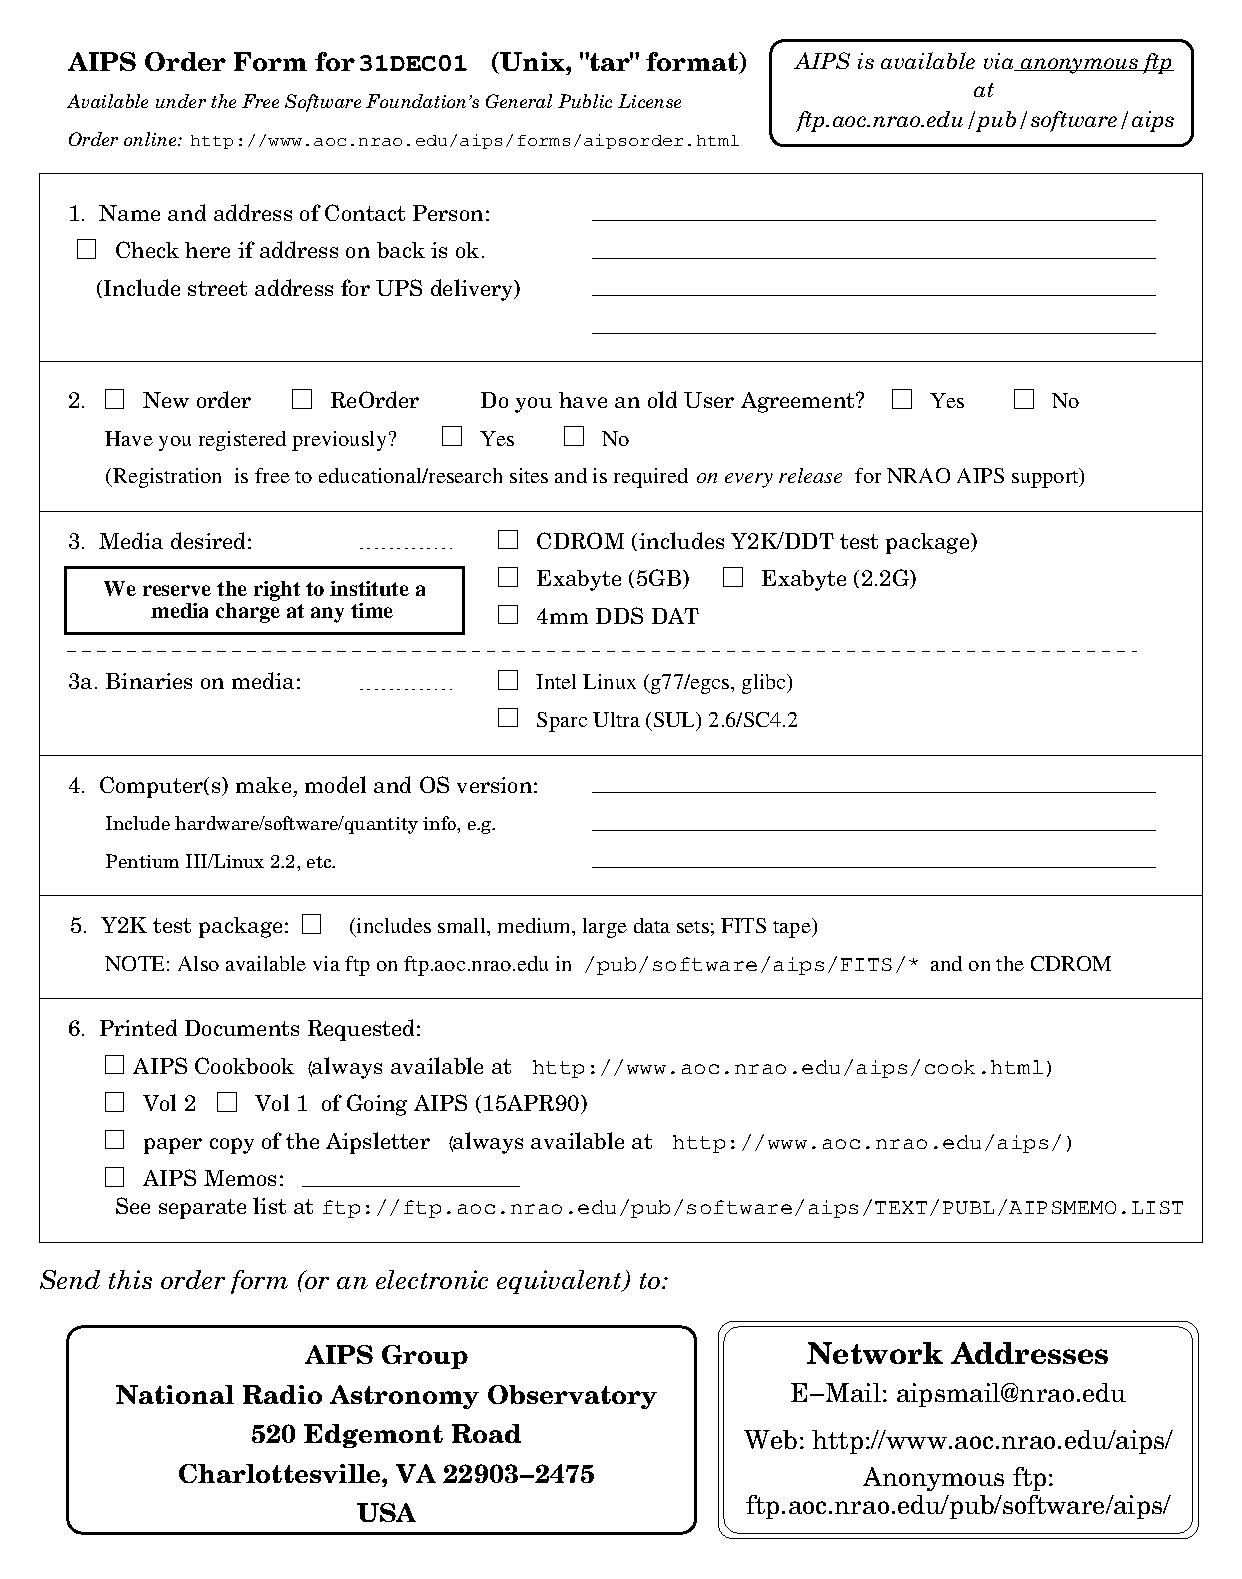
\includegraphics{FIG/AIPSORDER.PS}}}
% \vfill\eject
 \vbox to 4.4in{
  \vfill
  \centerline{\resizebox{!}{2.6in}{\includegraphics{FIG/Mandrill.eps}}}
  \vspace{12pt}
  \centerline{{\huge \tt \AIPRELEASE}}
  \vspace{12pt}
  \vfill}
\phantom{...}
\centerline{\resizebox{!}{!}{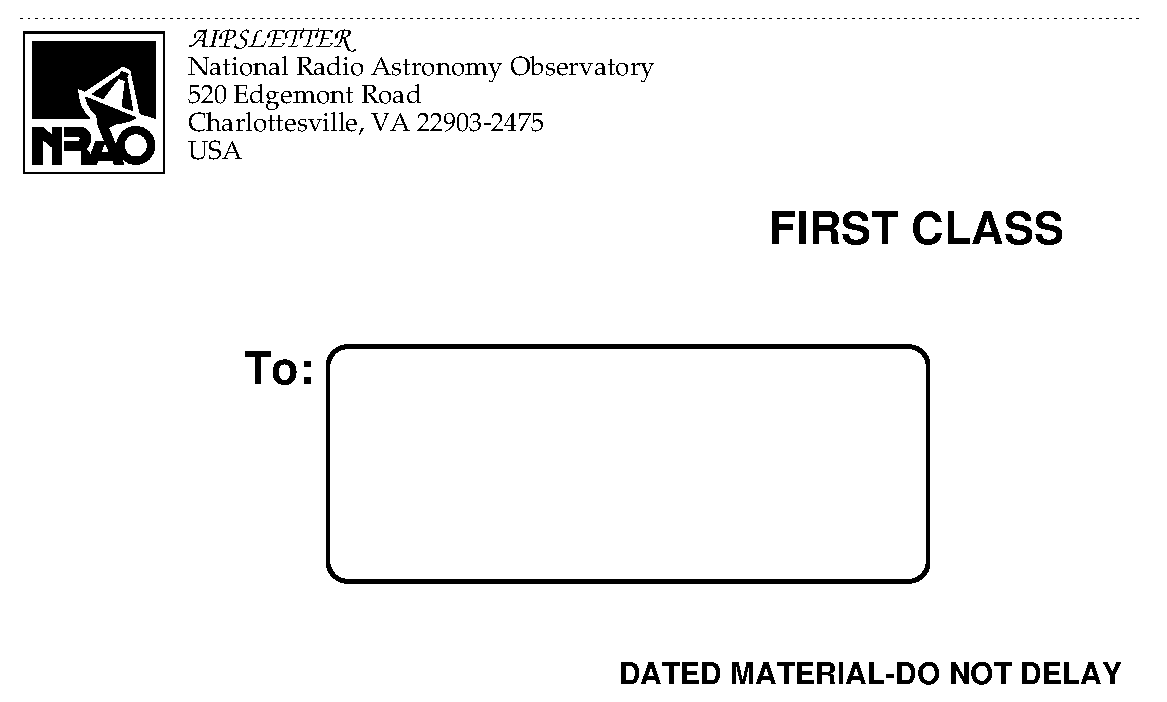
\includegraphics{FIG/AIPSLETM.PS}}}

\end{document}
